\documentclass[12pt]{article}
\usepackage{amsmath}
\usepackage{graphicx,psfrag,epsf}
\usepackage{enumerate}
\usepackage{enumitem}
\usepackage[numbers]{natbib}  % 使用 natbib,数字引用格式
\usepackage{booktabs}
\usepackage{tabularx}
\usepackage{array}
\newcommand{\blind}{0}

\addtolength{\oddsidemargin}{-.75in}%
\addtolength{\evensidemargin}{-.75in}%
\addtolength{\textwidth}{1.5in}%
\addtolength{\textheight}{1.3in}%
\addtolength{\topmargin}{-.8in}%

\begin{document}

\def\spacingset#1{\renewcommand{\baselinestretch}%
{#1}\small\normalsize} \spacingset{1}

%%%%%%%%%%%%%%%%%%%%%%%%%%%%%%%%%%%%%%%%%%%%%%%%%%%%%%%%%%%%%%%%%%%%%%%%%%%%%%

\if0\blind
{
  \title{\bf Enhancing Detection of Anomalies on IIoT Networks with Fine-tuned Large Language Models}
  \author{Huang Po-Hsun}
  \maketitle
} \fi

\if1\blind
{
  \bigskip
  \bigskip
  \bigskip
  \begin{center}
    {\LARGE\bf Title}
  \end{center}
  \medskip
} \fi

\bigskip
\begin{abstract}

  This research plan aims to enhance anomaly detection in Industrial Internet of Things (IIoT) networks by fine-tuning Large Language Models (LLMs). Addressing the limitations of current IoT systems in handling complex tasks and human interactions, as well as the shortcomings of the LLM-based task-oriented AI agent framework designed by Cui et al. (2024), which did not adequately consider network anomalies in IoT devices, this study proposes a new approach. Our goal is to leverage the time series learning capabilities of deep models to more accurately detect anomalous patterns, reduce false alarm rates, and construct an adaptable anomaly detection model suitable for various IoT scenarios and devices. By comparing with traditional detection methods, we expect the fine-tuned LLM to significantly improve the accuracy and efficiency of anomaly detection in IIoT networks, solving the problem of inadequate response to network anomalies in existing systems.

\end{abstract}

\noindent
{\it Keywords:}  IoT Device Control, Large Language Models, Intelligent Agents, IoT Networks

\spacingset{1.45}
\section{Background}
\label{sec:background}

  Blockchain technology and artificial intelligence (AI) have
emerged as two of the most transformative technologies of our
time \citep{zuo2024federated}.
On the other hand,
Large Language Models (LLMs) can understand and generate
human-like text, based on extensive training on diverse datasets
with billions of parameters \citep{kalita2024large}.
Task-oriented communications are an important
element in future intelligent Internet of Things (IoT) systems. Existing IoT systems,
however, are limited in their capacity to handle complex tasks,
particularly in their interactions with humans to accomplish these
tasks \citep{cui2024llmind}. 
The industry need to be good at making use of the LLM,
which has been popular in recent years, to improve
the shortcomings of the IoT in device networks.


\section{Objectives and Motivation}
\label{sec:objectives}
The continuous flow of data collected by IoT devices, has revolutionised
our ability to understand and interact with the world across various applications\citep{shirali2024llm}.
In Cui(2024), they Design an LLM-based taskoriented AI agent framework that enables effective collaboration
among IoT devices in Figure~\ref{fig:llmFramwork}\citep{cui2024llmind}.
However, although their system designed the conversion between natural language and code and executed it on IoT devices,
they did not further consider the problem of network anomalies in IoT devices.
This system is highly dependent on transmission between networks.
If a network failure occurs, there is no response to troubleshoot the problem.

And LLMs have provided highly effective methodologies and solutions
in various cybersecurity sectors \citep{mohamed2024efficient}.
As the frequency and diversity of cybersecurity attacks continue to rise, the
importance of incident detection has significantly increased \citep{thandi2024revolutionizing}.
Our goal is to more accurately detect abnormal patterns through the time series learning capabilities
of deep models. Use large models to understand multiple patterns to distinguish normal fluctuations from
abnormal situations and reduce false alarm rates.
Finally, an adaptable anomaly detection model is built that is suitable for a variety of IoT scenarios and devices.

\begin{figure}[h] % [h] 表示将图像放置在此处
  \centering
  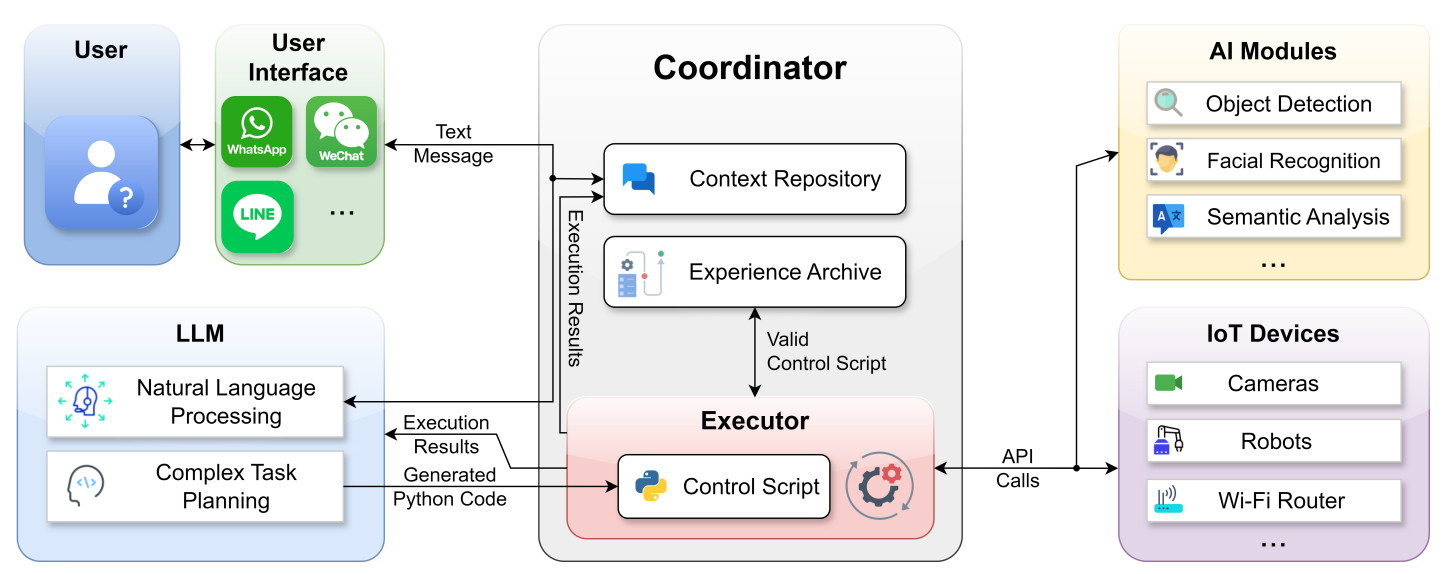
\includegraphics[width=0.7\textwidth]{./img/system_diagram.png} % 这里替换为图像文件名
  \caption{System diagram}
  \label{fig:llmFramwork}
\end{figure}

\section{Questions or Hypotheses}
\label{sec:questions}

  Below are posed to optimize network detection based on their designed IoT task-oriented framework,
  which may help identify potential challenges, define research directions,
  and evaluate the actual performance of the model:

\subsection{Questions}
\begin{enumerate}[label=\arabic*.]
  
  \item \textbf{Model Adaptability:} Can a large model, once fine-tuned, adapt to different IoT devices? In which device environments does it perform best?
  
  \item \textbf{Data Requirements:} Does fine-tuning an IoT anomaly detection model require a large amount of data? How do data scale and quality impact detection effectiveness?
  
  \item \textbf{Knowledge Base \& RAG Vector Database:} In Figure~\ref{fig:fsmProcedure}, if the RAG vector library and knowledge base are added, can the command problems of the system be better located? However, establishing this node requires additional resources.

  \begin{figure}[h] % [h] 表示将图像放置在此处
    \centering
    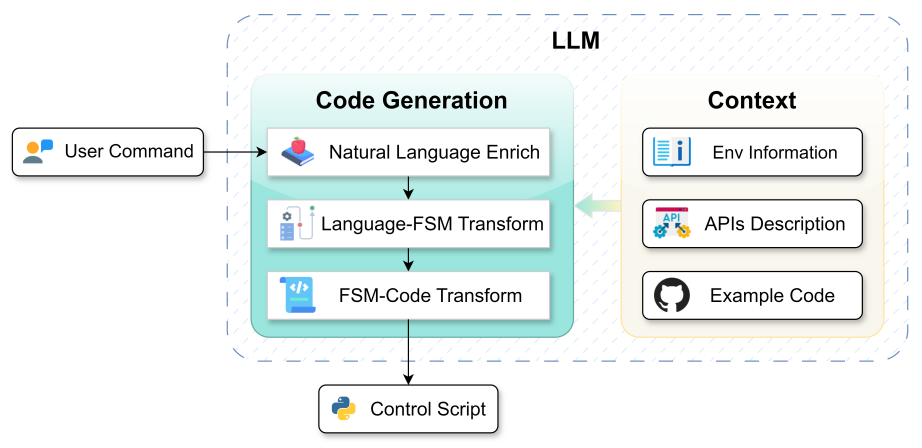
\includegraphics[width=0.7\textwidth]{./img/language_code_trans_procedure.png} % 这里替换为图像文件名
    \caption{Language-Code transformation procedure}
    \label{fig:fsmProcedure}
  \end{figure}

  \item \textbf{Real-time Detection:} Can the fine-tuned model meet real-time detection requirements in practical applications? If there is latency, how can it be optimized?
  
  \item \textbf{False Positive and False Negative Rates:} What are the model's false positive and false negative rates? How does detection accuracy vary across different types of anomalies, and are there specific anomaly types that are challenging to detect?
  
  \item \textbf{Resource Consumption:} What are the computational, storage, and energy costs when deploying the fine-tuned model in IoT environments? Can it effectively operate on resource-limited devices?
  
  \item \textbf{Model Scalability:} Can the model flexibly adapt to emerging IoT anomaly patterns, or does it require periodic fine-tuning or retraining?
  
  \item \textbf{Data Privacy:} How can IoT data privacy be effectively protected during data collection and model deployment?
\end{enumerate}

\subsection{Hypotheses}
\begin{enumerate}[label=\arabic*.]
  \item \textbf{H1:} Fine-tuning a large model significantly improves the accuracy and recall rates of IoT network anomaly detection, making it better suited for complex anomaly patterns than traditional detection methods.
  
  \item \textbf{H2:} A moderate amount of IoT anomaly data can greatly improve the model's generalization ability, enabling it to maintain high detection accuracy across various IoT environments.
  
  \item \textbf{H3:} Because in the industrial Internet of Things, the environment that isolates the external network needs to be considered, it is necessary to establish its own LLM independently. Compared with the resources consumed by running LLM, a vector library can be added to speed up the troubleshooting process.

  \item \textbf{H4:} The false positive rate of a fine-tuned large model will be substantially lower than traditional statistical or rule-based methods, thereby reducing interference in anomaly detection.
  
  \item \textbf{H5:} Distributed fine-tuning can effectively reduce the computational burden on IoT devices without significantly impacting detection performance.
  
  \item \textbf{H6:} The model’s accuracy in detecting new types of anomalies will degrade over time, but incremental fine-tuning can restore performance.
  
  \item \textbf{H7:} Multi-task fine-tuning (e.g., anomaly detection and classification in parallel) can further improve the model’s ability to identify specific types of anomalies.
  
  \item \textbf{H8:} The fine-tuned model is suitable for real-time anomaly detection, with a response time of 1-2 seconds for most IoT network anomalies.
\end{enumerate}

\section{Methodology}
\label{sec:methodology}

  The research will follow a systematic approach to develop and evaluate the proposed anomaly detection framework. The methodology includes the following steps:

\subsection{Technical Selection}
\begin{enumerate}[label=\arabic*.]
\item \textbf{Base Model:} Choose large language models or sequence modeling models that support network anomaly detection, such as OpenAI's GPT series or Hugging Face's BLOOM.
  \begin{itemize}
    \item \textbf{Specific Model Selection:} Models suitable for handling time series, such as T5, GPT, or transformer-based time series models, can be selected and fine-tuned for IoT data.
  \end{itemize}

  \item \textbf{Fine-Tuning Methods:}
  \begin{itemize}
    \item \textbf{Supervised Learning Fine-Tuning:} As shown in Table~\ref{tab:comparison}, Fine-tune the model using labeled normal/abnormal
    IoT network data to enable the model to recognize common anomaly patterns.
    
    \item \textbf{Reinforcement Learning from Human Feedback(RLHF) Fine-Tuning:} Further fine-tune the model using expert feedback after initial fine-tuning to optimize sensitivity to anomaly detection.
    The reward model for RLHF has proven effective in fine-tuning Large Language Models
    (LLMs)\citep{zhang2024prototypical}.
    
    \item \textbf{LoRA or Adapter:} SLoRA(2024) observe that this paradigm presents significant opportunities for batched inference during serving\citep{sheng2024slora}. We use LoRA for lightweight fine-tuning to save resources.
    
    \item \textbf{Mixture of Experts(Moe):} MoE is a model architecture that combines different experts (i.e., sub-models or networks) with the aim of activating only a subset of these "experts" based on the specific needs of the input task.
    LLM-HAS innovative framework leverages a Mixture
    of Experts (MoE) approach, augmented with LLMs, to analyze
    users’ personalized preferences and potential health risks from
    additional textual job descriptions\citep{gao2024guiding}.
  \end{itemize}

\begin{table}[h]
  \centering
  \fontsize{5}{8}\selectfont % 设置字体大小和行间距
  \begin{tabular}{@{}p{2cm}p{5cm}p{5cm}p{5cm}@{}} % 指定每列的宽度
      \toprule
      \textbf{Feature} & LoRA & RLHF & MoE \\ \midrule
      \textbf{Method Type} & Parameter-efficient fine-tuning & Training optimization & Model architecture \\
      \textbf{Core Goal} & Efficiently fine-tune the model & Enhance the quality of generated content through human feedback & Improve model performance through selective activation \\
      \textbf{Suitable Scenarios} & High task adaptability, minimal parameter adjustments needed & User interaction, dialogue systems & Multi-task learning, handling complex inputs \\
      \textbf{Advantages} & Resource-saving, lightweight fine-tuning & Aligns with human preferences, high-quality output & Large parameter count but controlled computational load \\
      \textbf{Implementation} & Low-rank matrix insertion & Reward model + reinforcement learning & Mixture of experts network + sparse activation \\
      \textbf{Cost} & Relatively low & Relatively high & High (but less computation during inference) \\
      \textbf{Complexity} & Low & High (involves human feedback and reinforcement learning) & High (requires expert selection and sparse activation) \\ 
      \bottomrule
  \end{tabular}
  \caption{Comparison of Different Methods}
  \label{tab:comparison}
\end{table}
  
\item \textbf{Supporting Tools:} The Hugging Face Transformers library and Datasets API can be used to handle datasets and model fine-tuning tasks; DeepSpeed can also be employed for distributed training and deployment.
\end{enumerate}

\subsection{Data Preparation}
\begin{enumerate}[label=\arabic*.]
  \item \textbf{Collecting IoT Data:} Gather traffic, logs, and sensor data from IoT devices over a period. Focus on collecting and labeling anomalies and normal events occurring in actual network environments.
  
  \item \textbf{Feature Extraction and Data Cleaning:} Extract features (e.g., traffic peaks, connection frequencies, packet sizes) from the data and remove noise. Data augmentation techniques can be used to expand anomaly samples.
  
  \item \textbf{Training Data Construction:} Organize data into time series input formats, such as sliding window sequences, for the model to learn inter-event relationships.
\end{enumerate}

\subsection{Model Fine-Tuning}
\begin{enumerate}[label=\arabic*.]
  \item \textbf{Phased Fine-Tuning:} We will select an appropriate LLM and fine-tune it on the collected IIoT data. As mentioned in the work of Touvron et al. (2023)\citep{sarabi2023llm}.First fine-tune the model using general network data to learn basic network patterns, then use IoT-specific data for further fine-tuning to learn specific patterns.
  
  \item \textbf{Multi-Task Training:} Implement multi-task learning to enable the model to perform anomaly detection while also classifying types of anomalies (e.g., identifying DDoS attacks, packet loss).
\end{enumerate}

\subsection{Evaluation and Validation}
\begin{enumerate}[label=\arabic*.]
  \item \textbf{Test Set Evaluation:} The fine-tuned LLM will be trained on the IIoT dataset, and its performance will be validated using a separate validation set to ensure the model's effectiveness in detecting anomalies.
  
  \item \textbf{Experimental Control:} Compare with traditional detection models (e.g., rule-based or statistical analysis methods) to analyze the advantages and shortcomings of the fine-tuned large model.
  
  \item \textbf{Comparison with Traditional Methods:} The performance of the fine-tuned LLM will be compared with traditional anomaly detection methods to evaluate its improvement in accuracy and efficiency.

  \item \textbf{Real-world Implementation and Testing:} The model will be deployed in a real-world IIoT network setting to test its practical applicability and robustness in various operational scenarios.
\end{enumerate}

\section{Expected Outcomes and Contributions}
\label{sec:outcomes}

  We expect the fine-tuned LLM to significantly enhance the accuracy and efficiency of anomaly detection in IIoT networks. The successful implementation of this research will contribute to the following:

\begin{enumerate}[label=\arabic*.]
  \item \textbf{A Novel Anomaly Detection Framework:} A new framework that leverages the power of LLMs for IIoT security, providing a more proactive approach to threat detection.

  \item \textbf{Improved Security and Resilience:} Enhanced security measures for IIoT networks, leading to increased resilience against potential threats and anomalies.

  \item \textbf{Advancing LLM Applications:} Expanding the application domain of LLMs in industrial settings, demonstrating their versatility beyond natural language tasks.

  \item \textbf{Empirical Evidence:} Providing empirical evidence on the effectiveness of fine-tuned LLMs in improving IIoT network security, contributing to the body of knowledge in this emerging field.
  
  \item \textbf{Improved Detection Accuracy:} The model should achieve high accuracy and recall rates post fine-tuning, with expected accuracy improvements of 5-10\%.
  
  \item \textbf{Enhanced Real-Time Responsiveness:} Achieve real-time response in anomaly detection through distributed deployment.
  
  \item \textbf{Improved Anomaly Pattern Recognition Ability:} The model will adapt more quickly to new or complex anomalies, expanding its ability to detect different types of attacks or anomalies.
  
  \item \textbf{Scalability:} Maintain the model's adaptability to emerging IoT anomalies through periodic fine-tuning or the use of new data.
\end{enumerate}

\textbf{Example Application Scenario:} In a home monitoring network, the fine-tuned model can identify anomalies such as sudden bandwidth spikes or frequent packet losses, alerting users to potential network intrusions or device anomalies in a timely manner. This helps in proactively preventing and reducing IoT security risks.

\bibliographystyle{unsrtnat} % 选择 natbib 支持的引用样式
\bibliography{references} % 使用 references.bib 文件,不要加 .bib 后缀

\end{document}
